%%-------------------------process on a circle---------------------------------------%%
\blue{
	discuss about data generation on a circle, 
	\begin{itemize}
		\item including circulant matrix
		\item why circulant matrix
		\item discuss covarince, biasness and the difficulties of estimation
		\item discuss variogram
		\item jones 1963
	\end{itemize}
}

%%------------------------------------------------------------------%%
\section{Circulant matrix}
%%------------------------------------------------------------------%%

A square matrix $A_{n\times n}$ is a circulant matrix if the elements of each row (except first row) has the previous row shifted by one place to the right.

\begin{eqnarray}
	A = circ[a_o, a_1,\cdots,a_{n-1}] &=& \left[
		\begin{array}{lllll}
			a_0     & a_1     & a_2    & \cdots & a_{n-1} \\
			a_{n-1} & a_0     & a_1    & \cdots & a_{n-2} \\
			a_{n-2} & a_{n-1} & a_0    & \cdots & a_{n-3} \\
			\vdots  & \vdots  & \vdots & \ddots & \ldots  \\
			a_1     & a_2     & a_3    & \cdots & a_0     
		\end{array}
	\right].
\end{eqnarray}

The eigenvalues of $A$ are given by
\[
	\lambda_l = \sum_{k=0}^{n-1} a_k e^{-i2lk\pi/n} = \sum_{k=0}^{n-1}c_k \rho_l^k, \quad \quad l = 0, 1, 2, \cdots, n-1,
\]
($\rho_l = e^{-i2\pi l/n}$ represents the $l$th root of 1), and the corresponding (unitary) eigenvector is given by
\[
	\psi_l = \frac{1}{\sqrt{n}}(1, \rho_l, \rho_l^2, \cdots, \rho_l^{n-1})^T.
\]

\blue{should we talk more about hermitian, and block circulant matrices?}

%%------------------------------------------------------------------%%
\section{Stationary process on a circle}
%%------------------------------------------------------------------%%

Let $\{X(t_k), k = 1, 2, \cdots, n\}$ be a collection of gridded observations on a circle, with $t_k = (k-1)*2\pi/n, k = 1, 2, \cdots, n$. Lets assume $E(X(t)) = \mu$ is unknown, the unbiased estimator of $\mu$ is given by $\bar{X} = \frac{1}{n}\sum_{i=1}^{n} X(t_i)$. The underlying process is stationary, if it's covariance function solely depends on the distance $\theta$,
\beq
C(\theta) = cov(X(t+\theta), X(t)), \quad \quad \theta \in [0, \pi].
\eeq
The spectral representation for $C(\theta)$ is given by
\beq
C(\theta) = a_0 + \sum_{k = 1}^\infty a_k \cos(k \theta), \quad \theta \in [0, \pi].
\eeq 

%%------------------------------------------------------------------%%
\section{Estimation}
%%------------------------------------------------------------------%%

%-------------------------------------% 
\subsection{Estimation of covaraince on a cricle}
%-------------------------------------%

We used method of moments (MOM) to estimate the covariance $C(\theta)$ on a circle, the estmator can be given by

\beq
\hat{C}(\Delta \lambda) = \frac{1}{n}\sum_{i = 1}^n (X(t_i + \Delta \lambda) - \bar{X})(X(t_i) - \bar{X}), 
\eeq

where $\Delta \lambda = 0, 2\pi/n, 4\pi/n, \cdots, 2(N-1)\pi/n$.\\

Now we shall check the unbiasedness and consistency of the above estimator.

\begin{eqnarray}
	\nonumber
	E(\hat{C}(\Delta \lambda)) &=& \frac{1}{n}\sum_{i = 1}^n E((X(t_i + \Delta \lambda) - \bar{X})(X(t_i) - \bar{X})) \\ \nonumber
	&=& \frac{1}{n}\sum_{i = 1}^n E((X(t_i + \Delta \lambda) - \mu - (\bar{X} - \mu))(X(t_i) -\mu - (\bar{X}) - \mu)) \\ \nonumber
	&=& \frac{1}{n}\sum_{i=1}^n cov(X(t_i+\Delta \lambda), X(t_i)) - \frac{1}{n}\sum_{i = 1}^n E((X(t_i + \Delta \lambda) - \mu)(\bar{X} - \mu)) \\ \nonumber
	& & -\frac{1}{n}\sum_{i = 1}^n E((X(t_i) - \mu)(\bar{X} - \mu)) + \frac{1}{n}\sum_{i = 1}^n E((\bar{X} - \mu)(\bar{X} - \mu)) \\ \nonumber
	&=& C(\Delta \lambda) -E((\bar{X} - \mu)(\bar{X} - \mu)) - E((\bar{X} - \mu)(\bar{X} - \mu)) + E((\bar{X} - \mu)(\bar{X} - \mu)) \\ 
	&=& C(\Delta \lambda) - var(\bar{X}).
\end{eqnarray}

Moreover,

\begin{eqnarray*}
	\nonumber
	var(\bar{X}) &=& E((\bar{X} - \mu)(\bar{X} - \mu)) = \frac{1}{n^2}\sum_{i = 1}^n \sum_{j=1}^n E(X(t_i) - \mu)(X(t_j) - \mu) \\ \nonumber
	&=&  \frac{1}{n^2}\sum_{i = 1}^n \sum_{j=1}^n cov(X(t_i), X(t_j)) = \frac{1}{n^2}\sum_{i = 1}^n \sum_{j=1}^n C(m*(i-j)*2\pi/n) \\ \nonumber
	&=& \frac{1}{n^2}\sum_{i = 1}^n \sum_{j=1}^n \left(a_0 + \sum_{k=1}^\infty a_k \cos(m*(i-j)*2\pi/n)\right) \\ \nonumber
	&=& a_0 + \sum_{k=1}^\infty a_k \left(\frac{1}{n^2}\sum_{i = 1}^n \sum_{j=1}^n \cos(m*(i-j)*2\pi/n)\right).
\end{eqnarray*}

Now,

\begin{eqnarray*}
	& & \sum_{i = 1}^n \sum_{j=1}^n \cos(m*(i-j)*2\pi/n) \\
	&=& \sum_{i=1}^n \sum_{j=1}^n \left(\cos(m*i *2\pi/n)\cos(m*j*2\pi/n) + \sin(m*i *2\pi/n)\sin(m*j*2\pi/n) \right)\\
	&=& \left(\sum_{i=1}^n \cos(m*i *2\pi/n)\right)^2 + \left(\sum_{i=1}^n \sin(m*i *2\pi/n)\right)^2 = n^2
\end{eqnarray*}

since for any integer $m$, we have

\[
	\sum_{k = 1}^{n} \cos(mk*2\pi/n) = \left\{\begin{array}{cc}
	0, & \mbox{for any integer $m \ne 0$,}  \\
	n, & \mbox{for $m = 0$}
	\end{array}
	\right. \mbox{ and }
	\sum_{k = 1}^{n} \sin(mk*2\pi/n) = 0.
\]

Hence,
\[
	var(\bar{X}) = a_0.
\]

Therefore,
\beq
E(\hat{C}(\Delta \lambda)) = C(\Delta \lambda) - a_0.
\eeq

That is, the MOM estimator $\hat{C}(\Delta \lambda)$ of the covariance function is actually a biased estimator with the shift amount of $a_0$. Therefore, if $a_0 = 0$ for a covariance function, we have the unbiased estimator $\hat{C}(\Delta \lambda)$. \\

If $a_0 = 0$ implies that $var(\bar{X}) = 0 \Rightarrow \bar{X} = \mu$ a.s., which might not be practically possible. On the other hand, if $a_0 \ne 0$, then $var(\bar{X}) \ne 0$. This indicates that $\bar{X}$ will never be a consistent estimator for $\mu$ regardless of the sample size $n$.\\

If the gridded points were on a line, for example in time series, $E(\bar{X} - \mu)^2 \to 0$ as $n \to \infty$ under the assumption that the covariance function $C(\theta) \to 0$ when $\theta \to \infty$ (which is practically feasible), that is, $\bar{X}$ is consistent in the case of points on a line. In the case of circle, we might not have $C(\theta)$ close to 0 since $\theta$ is within a bounded region ($(0, \pi)$ for the circle) and we normally assume $C(\theta)$ is continuous for $\theta$. \\

%-------------------------------------%
\subsection{Estimation of variogram on a circle}
%-------------------------------------%

The theoretical variogram function is given by,
\beq
\gamma(\theta) = C(0) - C(\theta).
\eeq
 and the MOM estimator for the variogram is given by,

\beq
\hat{\gamma}(\Delta \lambda) = \frac{1}{2n} \sum_{i=1}^n (X(t_i + \Delta \lambda) - X(t_i))^2.
\eeq

We can show that variogram estimator through MOM is an unbiased estimator, 

\begin{eqnarray*}
E(\hat{\gamma}(\Delta \lambda)) &=& \frac{1}{2n} \sum_{i = 1}^n E(X(t_i + \Delta \lambda) - X(t_i))^2 \\
&=& \frac{1}{2n} \sum_{i = 1}^n E((X(t_i + \Delta \lambda)-\mu) - (X(t_i) - \mu))^2 \\
&=& \frac{1}{2n} \sum_{i = 1}^n cov(X(t_i + \Delta \lambda) - X(t_i), X(t_i + \Delta \lambda) - X(t_i)) \\
&=& \frac{1}{2n} \sum_{i = 1}^n \left\{ cov(X(t_i + \Delta \lambda), X(t_i + \Delta \lambda)) + cov(X(t_i), X(t_i)) \right. \\
& & \left. - 2cov(X(t_i + \Delta \lambda), X(t_i)) \right\}\\
&=& \frac{1}{2n} \sum_{i = 1}^n \left( C(0) + C(0) - 2C(\Delta \lambda)\right) \\
&=& C(0) - C(\Delta \lambda) = \gamma(\Delta \lambda).
\end{eqnarray*}
% 
% \blue{need to prove consistency}


%-------------------------------------%
%-------------------------------------% 
\section{Data generation on a circle}

Using the covarince function $C_1e^{-a|\Delta\lambda|}$ and estimate empirical covarince from MOM as follows,

\beq\label{cov:circle1}
C(\theta) = \frac{1}{n_L} \sum_{i=1}^{n_L} (X(a_i+\theta)\cdot X(a_i))-(\overline{X(a)})^2
\eeq


\begin{figure}
	\centering
	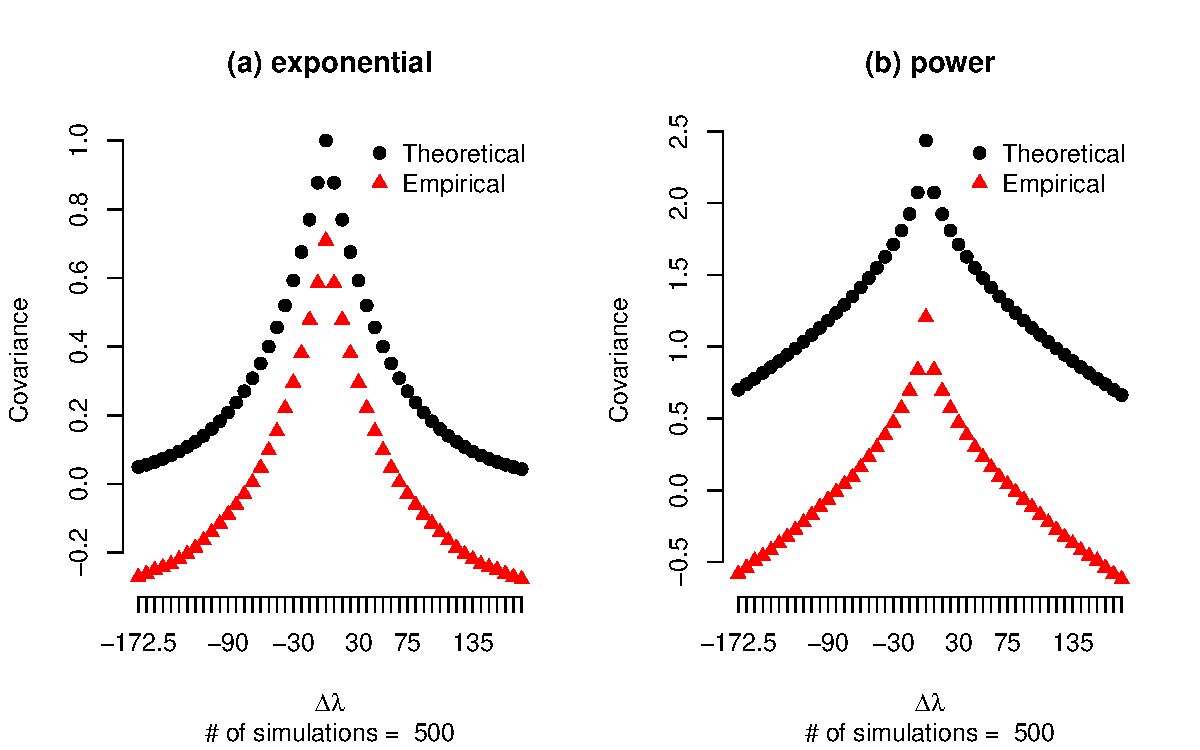
\includegraphics[width=0.65\textwidth]{graphs/covarince_circle}
	\caption {Theoretical and empirical covariance comparison comparison on a circle}
\end{figure}


\begin{figure}
	\centering
	%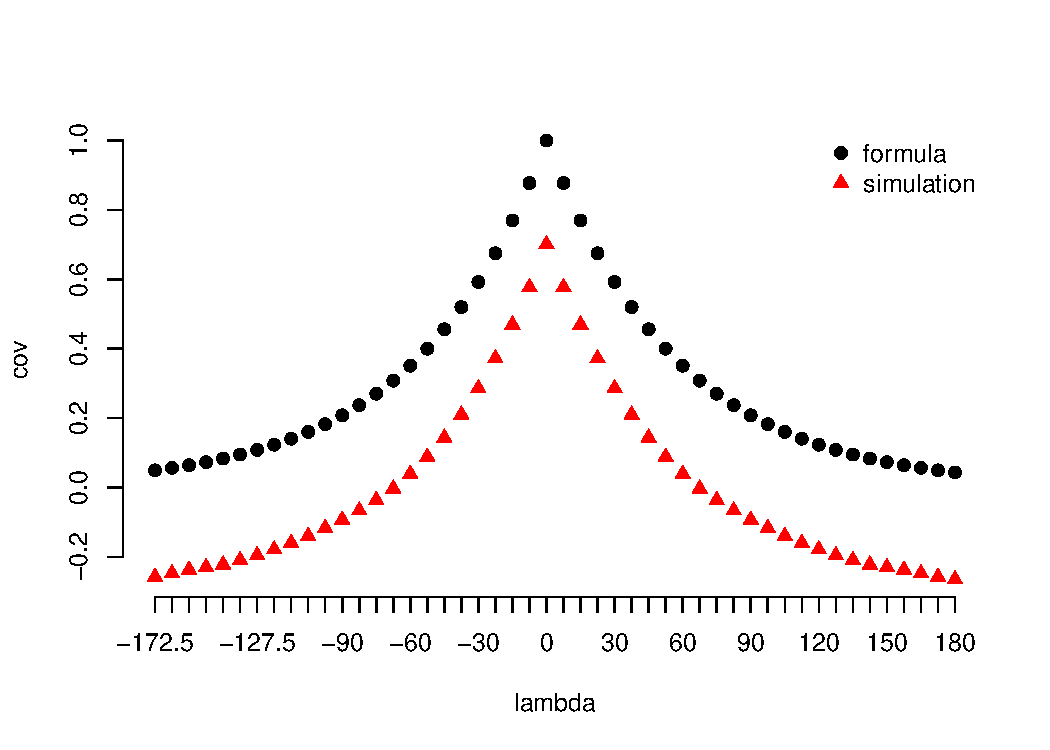
\includegraphics[width=0.65\textwidth]{graphs/Summary-covarince_circle_1}
	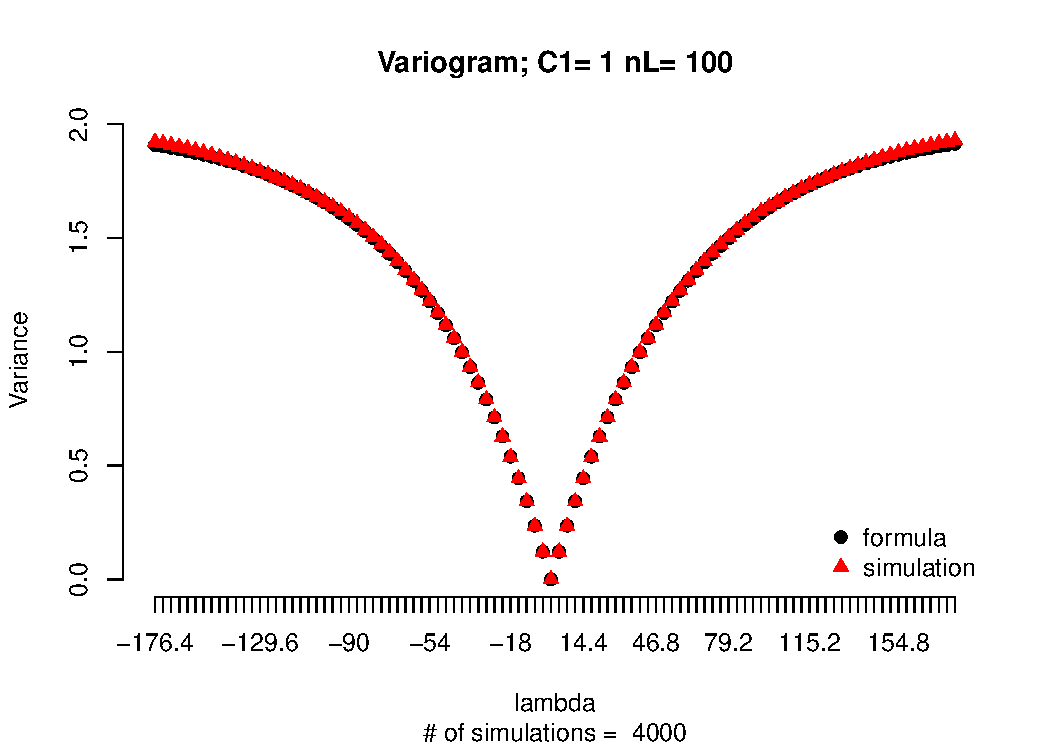
\includegraphics[width=0.65\textwidth]{graphs/variogram_plot_4000}
	%graph from data genaration summary doc line 177 
	\caption {Theoretical and empirical covariance comparison comparison on a circle}
\end{figure}

covariance estimator without the mean term

\beq \label{cov:circle1}  
C(\theta) = \frac{1}{n_L} \sum_{i=1}^{n_L} (X(a_i+\theta) \cdot X(a_i)) 
\eeq

\begin{figure}
	\centering
	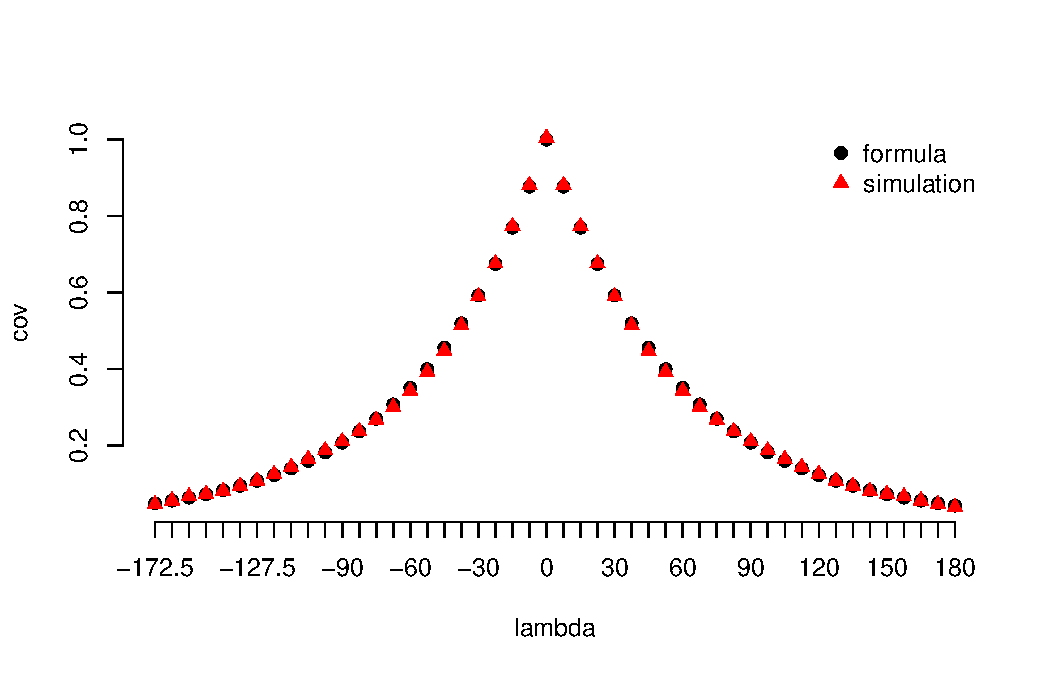
\includegraphics[width=0.65\textwidth]{graphs/Summary-covarince_circle_2}
	%graph from data genaration summary doc line 194 
	\caption {Theoretical and empirical covariance comparison comparison on a circle}
\end{figure}